\documentclass[a4paper,titlepage]{article}
\usepackage{amssymb}
\usepackage[OT4,plmath]{polski}
\usepackage[polish]{babel}
\usepackage{csquotes}
\DeclareQuoteAlias{croatian}{polish} % cudzysłowy w bibliografii
\usepackage[style=numeric,sorting=nty,isbn=false,abbreviate = false,backend=biber]{biblatex}
\usepackage[margin=1in]{geometry}
\usepackage[noend]{algpseudocode}
\usepackage[page]{appendix}
\usepackage[usenames,dvipsnames,svgnames,table]{xcolor}
\usepackage[utf8]{inputenc}
\usepackage{adjustbox}
\usepackage{algorithm}
\usepackage{amsfonts}
\usepackage{amsmath}
\usepackage{amsthm}
\usepackage{array}
\usepackage{enumitem}
\usepackage{graphicx}
\usepackage{hyperref}
%\usepackage{indentfirst}
\usepackage{longtable}
\usepackage{multirow}
\usepackage{parskip}
\usepackage{pifont}
\usepackage{setspace}
\usepackage{verbatimbox}
\usepackage{wrapfig}
\usepackage{bm}
\usepackage{mathtools}
\usepackage{afterpage}
\usepackage{listings}
\usepackage{csquotes}

\newcommand\blankpage{%
	\null
	\thispagestyle{empty}%
	\addtocounter{page}{-1}%
	\newpage}

\linespread{1.4}

\renewcommand*\appendixpagename{Załącznik}
\renewcommand{\qedsymbol}{$\square$}
\renewcommand{\algorithmiccomment}[1]{\hfill\textcolor{black!65}{\textit{#1}}}
\let\emptyset\varnothing

\makeatother
%\setlength{\parindent}{24pt}
\theoremstyle{break}
\newtheorem*{uwaga}{Uwaga}
\newtheorem{definicja}{Definicja}[section]
\newtheorem{ozn}{Oznaczenie}[section]

\newcommand{\cmark}{\textcolor{ForestGreen}{\ding{51}}}
\newcommand{\xmark}{\textcolor{Maroon}{\ding{55}}}

\numberwithin{equation}{subsection}
\addbibresource{Dokumentacja.bib}

%------------------------------------------------------------------------------

\title{Dokumentacja projektu\\[0.6em]Identyfikacja twarzy}
\author{
    \href{mailto:bezap@student.mini.pw.edu.pl}{inż.~Patryk~Bęza}\\[0.7em]
    \href{mailto:kozakm@student.mini.pw.edu.pl}{inż.~Marek~Kozak}\\[0.7em]
    \href{mailto:malasnickik@student.mini.pw.edu.pl}{inż.~Krzysztof~Małaśnicki}\\[0.7em]
}
\date{\today}

\begin{document}

\makeatletter
\renewcommand{\ALG@name}{Algorytm}
\begin{titlepage}
\newcommand{\HRule}{\rule{\linewidth}{0.5mm}}
\center


\includegraphics[width=2.0cm]{img/mini}\\[1.5cm]
\textsc{\LARGE Politechnika Warszawska}\\[0.3cm]
\textsc{\Large Wydział Matematyki i~Nauk Informacyjnych}\\[1.5cm]
\textsc{\large Komputerowe wspomaganie technik kryminalistycznych}\\[0.2cm]
\textsc{\small Rok akademicki 2015/2016}\\[1.5cm]

\HRule \\[0.7cm]
{ \huge \bfseries \@title}\\[0.7cm]
\HRule \\[1.75cm]

\begin{minipage}[t]{0.4\textwidth}
\begin{flushleft}\large
\textsc{Autorzy:}\\[3mm]
\@author
\end{flushleft}
\end{minipage}
\begin{minipage}[t]{0.4\textwidth}
\begin{flushright}\large
\textsc{Wykładowca:}\\[3mm]
\href{mailto:m.szezynska@ise.pw.edu.pl}{dr~inż.~Magdalena~Szeżyńska}\\[1cm]
\end{flushright}
\end{minipage}
\vfill
{\large \today}

\end{titlepage}

%\maketitle
\blankpage
\tableofcontents
\clearpage
\blankpage

%------------------------------------------------------------------------------

\begin{abstract}

\begin{figure}[t]
    \centering
    \hspace{-2em}
    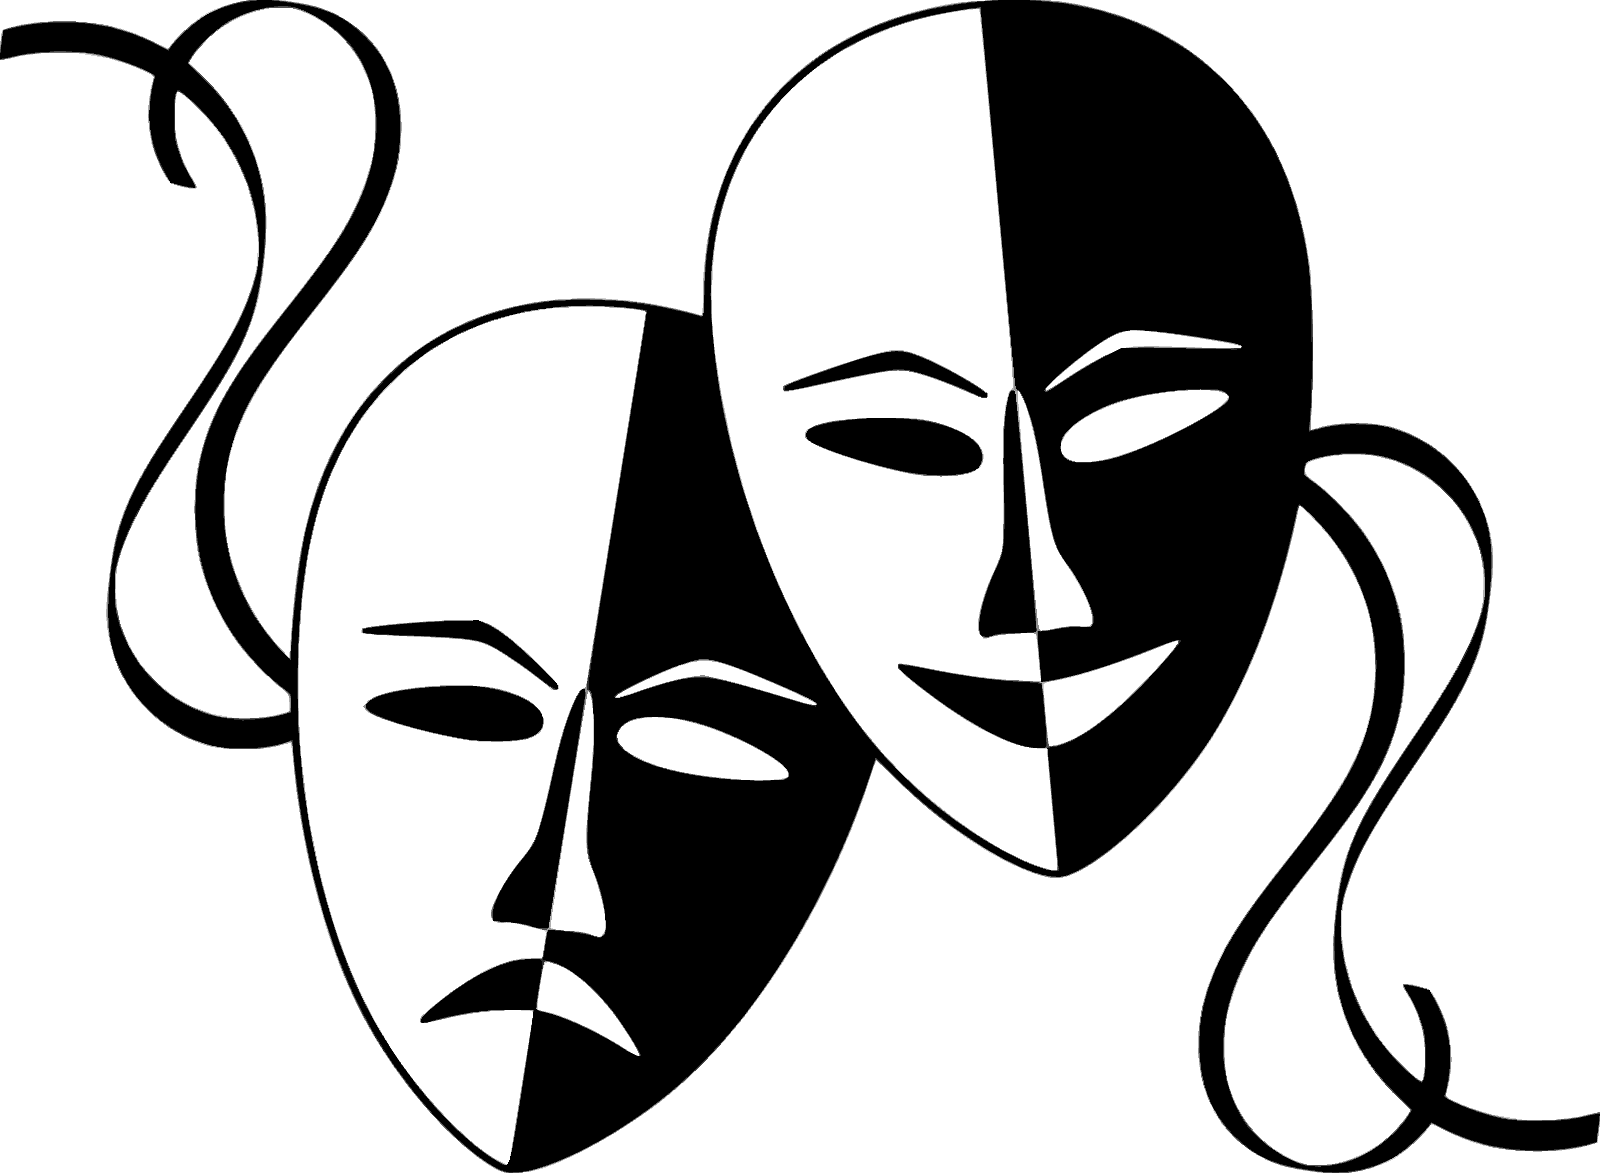
\includegraphics[width=0.45\textwidth]{img/faces}
\end{figure}

Niniejszy dokument powstał w~ramach dokumentacji projektu zespołowego z~przedmiotu \emph{\href{http://staff.elka.pw.edu.pl/~mszezyns/CAF/index.html}{Komputerowe wspomaganie technik kryminalistycznych}} w semestrze letnim roku akademickiego~2015/2016 na \emph{\href{http://www.mini.pw.edu.pl/}{Wydziale MiNI}~\href{https://www.pw.edu.pl/}{Politechniki Warszawskiej}}. Ma on za zadanie udokumentować ideę działania aplikacji identyfikującą twarze, uzasadnienie wyboru zastosowanych algorytmów, sposób jej użycia, wykorzystane narzędzia i biblioteki, wyniki testów oraz wnioski.

\end{abstract}

\clearpage

%------------------------------------------------------------------------------

\section{Wstęp}
\label{sec:wstep}

W tym rozdziale przedstawiono założenia wstępne projektu pt.~,,Identyfikacja twarzy".

%------------------------------------------------------------------------------

\subsection{Identyfikacja twarzy}

Identyfikacja twarzy to przypisanie tożsamości do dwu- lub trójwymiarowego zdjęcia twarzy. Przez ostatnie kilkadziesiąt lat opracowano wiele algorytmów, które służą do rozpoznawania i identyfikacji twarzy. Część z nich jest oparta na sieciach neuronowych, a pozostała część korzysta z klasycznych metod aparatu matematycznego, np. algebry i analizy statystycznej.

W ramach niniejszego projektu powstało rozwiązanie oparte o metody klasyczne, oparte na algebrze, a w szczególności na wyliczaniu wartości własnych i wektorów własnych macierzy, powstałej z analizowanych zdjęć twarzy, celem zamodelowania analizowanych zdjęć w przestrzeni liniowej, rozpiętej przez wyliczone wektory własne. Wykorzystana metoda identyfikacji twarzy to metoda~\emph{eigenfaces}, która opiera się na metodzie analizy głównych składowych~(ang.~\emph{Principal Component Analysis} -- w~skrócie:~PCA).

%------------------------------------------------------------------------------

\subsection{Zastosowania identyfikacji twarzy}

Istnieje wiele zastosowań identyfikacji twarzy. Część z nich dotyczy zastosowań w rozrywce, takiej jak np. gry czy identyfikacja twarzy na zdjęciach serwisów społecznościowych\footnote{W przeciwieństwie do rozpoznawania twarzy, identyfikacja twarzy nie jest jeszcze stosowana na szeroką skalę na największych serwisach społecznościowych.}. Poza zastosowaniami identyfikacji twarzy w rozrywce, istnieją zastosowania do poważniejszych celów, np. do wspomagania technik kryminalistycznych i szeroko pojętego bezpieczeństwa danych, np.: systemy kontroli dostępu, systemy bezpieczeństwa na lotniskach, policyjne bazy danych osób poszukiwanych (np. zaginionych, poszukiwanych listami gończymi i podejrzanych).

Identyfikacja twarzy w komputerowym wspomaganiu technik kryminalistycznych jest ważnym zagadnieniem dla wszystkich służb dbających o bezpieczeństwo, które posiadają bazy danych ze zdjęciami twarzy tysięcy osób, wśród których może znajdować się zdjęcie osoby identyfikowanej, np. podejrzanej, winnej, poszukiwanej lub zaginionej. Niniejsza dokumentacja jest opisem szczegółów implementacyjnych aplikacji służącej do identyfikacji dwuwymiarowych zdjęć twarzy.

%------------------------------------------------------------------------------

\subsection{Cel aplikacji}

Celem aplikacji tworzonej w ramach niniejszego projektu jest zidentyfikowanie zadanej twarzy na podstawie zbioru zdjęć osób z lokalnej bazy danych. Zakładamy, że zdjęcia są znormalizowane, tzn. wszystkie zdjęcia są monochromatyczne, mają jednakowe rozmiary, twarze sfotografowana są frontalnie, tzn.~\emph{en~face} i są wycentrowane.

Jeśli osoba, której twarz podano na wejście programu nie znajduje się w bazie danych, program powinien zwrócić kilka zdjęć najbardziej podobnych do zadanego wraz z oszacowaniem ich podobieństwa w skali od $0\%$ do $100\%$ lub w innej mierze odległości. W obu przypadkach zdjęcia znalezionych twarzy powinny być posortowane nierosnąco względem podobieństwa do zadanej twarzy.

W przeciwnym razie, tzn. jeśli zdjęcia osoby, której twarz została poddana identyfikacji, znajdują się w bazie danych, program powinien znaleźć tę twarz i przypisać wartość jej podobieństwa bliską $100\%$ (wartość oczekiwana $=100\%$) oraz ewentualnie kilka innych, podobnych twarzy, z odpowiednio mniejszym podobieństwem wyrażonym w skali od $0\%$ do $100\%$ lub innej mierze odległości.

Pierwszorzędnym celem aplikacji \emph{nie} jest szybkie działanie, co można uzasadnić tym, że algorytmy mające na celu zidentyfikowanie osoby, powinny przede wszystkim nie dopuścić do przeoczenia osoby, która znajduje się w bazie danych. Tak postawione wymaganie na ogół wymusza zastosowania algorytmów, które działają względnie długo.

%------------------------------------------------------------------------------

\section{Algorytm}
\label{sec:algorytm}

Do rozpoznawania twarzy została zastosowana \emph{metoda analizy głównych składowych}~(ang.~\emph{Principal Component Analysis} -- w~skrócie:~PCA), zaproponowana niezależnie przez angielskiego matematyka \emph{Karla Pearson'a}~(1901) oraz ekonoma i statystyka \emph{Harolda Hotelling'a}~(1933).

W niniejszym dziale przedstawiono uzasadnienie wyboru algorytmu, opis metody PCA oraz \emph{eigenfaces}, na podstawie publikacji autorów metody \emph{eigenfaces} -- prof.~\emph{Matthew Turk'a} i prof.~\emph{Alex'a Pentland'a}\cite{turk}.

%------------------------------------------------------------------------------

\subsection{Analiza głównych składowych}

Jednym z głównych problemów z jakim mamy do czynienia w identyfikacji twarzy ze zdjęć, jest ich duży wymiar. Dwuwymiarowe, monochromatyczne zdjęcie zdjęcie o wymiarach $p\times q$, rozpina przestrzeń $m=p\cdot q$--wymiarową. Zdjęcie o wymiarach $100\times 100$~pikseli, rozpina przestrzeń $10000$-wymiarową. Istnieje potrzeba zmniejszenia tej przestrzeni kosztem możliwie małych różnic między oryginalnym zdjęciem, a zdjęciem reprezentowanym w ,,skompresowanej" przestrzeni liniowej. Okazuje się, że do celów identyfikacji twarzy, nie wszystkie wymiary/osie są jednakowo istotne. Będziemy chcieli zachować tylko te wymiary, dla których wariancja jest największa, tak, aby skutecznie rozróżniać zdjęcia twarzy, korzystając z możliwie najmniejszej ilości wymiarów\cite{www:opencv}.

Główna idea metody \emph{eigenfaces}, to przedstawienie zdjęcia jako liniowa kombinacja obrazów bazowych~(patrz równanie~\ref{eq:eigenfaces}), zapisywanych w postaci wektorów, nazywanych również~\emph{eigenfaces}. Dzięki temu obraz możemy przestawić w zwartej postaci wektora $[\omega_1,\dotsc,\omega_M]$, o długości znacznie mniejszej od wymiaru obrazu~$N^2$.

Załóżmy, że mamy zbiór zdjęć twarzy treningowych, pobranych z bazy danych, w postaci $M$ wektorów $\bm{\Gamma_1},\bm{\Gamma_2},\dotsc,\bm{\Gamma_M}$, z których każdy ma długość $N\cdot N$, gdzie $N$ to długość i wysokość zdjęcia\footnote{Dla uproszczenia oznaczeń w opisie metody, zakładamy, że wysokość zdjęcia jest równa szerokości zdjęcia.}. Średnia twarz tego zbioru twarzy testowych jest zdefiniowana jako następujący wektor $\bm{\Psi}$ o długości $N\cdot N$:
\begin{equation}
	\bm{\Psi}=\frac{1}{M}\cdot\sum\limits_{n=1}^M\bm{\Gamma_n}
\end{equation}
$i$-ta twarz treningowa $\bm{\Gamma_i}$ różni się od twarzy średniej $\bm{\Psi}$ o pewien wektor $\bm{\Phi_i}$:
\begin{equation}
	\bm{\Phi_i}=\bm{\Gamma_i}-\bm{\Psi}
\end{equation}
Zbiór wektorów $\{\bm{\Phi_1},\bm{\Phi_2},\dotsc,\bm{\Phi_M}\}$ poddajemy metodzie \emph{analizy głównych składowych}, dzięki której otrzymamy zbiór $M$ ortonormalnych\footnote{Ortonormalnych, czyli jednocześnie ortogonalnych i normalnych.} wektorów $\{\bm{u_1},\bm{u_2},\dotsc,\bm{u_M}\}$, które najlepiej obrazują rozkład wartości pikseli. $k$-ty wektor $\bm{u_k}$ jest wybierany tak, aby:
\begin{equation}
	\bm{\lambda_k}=\frac{1}{M}\cdot\sum\limits_{n=1}^M(\bm{u_k^T}\bm{\Phi_n})^2
\end{equation}
był maksymalny gdzie\footnote{$\delta_{lk}$ jest nazywana deltą lub symbolem \emph{Kroneckera}.}:
\begin{equation}
\label{ortogonalnosc}
	\bm{u_l^T}\bm{u_k}=\delta_{lk}=
	\begin{cases}
		1,&\text{gdy }l=k\\
		0,&\text{gdy }l\neq k
	\end{cases}
\end{equation}
Równanie \ref{ortogonalnosc} mówi, że każde dwa, różne wektory $\bm{u_k}$, $\bm{u_l}$, gdzie $k\neq l$, są ortogonalne względem siebie. Wektory $\bm{u_k}$ i skalary $\lambda_k$ to odpowiednio wektory własne i wartości własne następującej macierzy kowariancji:
\begin{equation}
	C=\frac{1}{M}\cdot\sum\limits_{n=1}^M\bm{\Phi_n}\bm{\Phi_n^T}=AA^T
\end{equation}
gdzie:
\begin{equation}
	A=[\bm{\Phi_1}\bm{\Phi_2}\dotsc\bm{\Phi_M}]
\end{equation}
Rozmiar macierzy $C$ jest bardzo duży -- wynosi $N^2\times N^2$. Liczenie $N^2$ wartości własnych i wektorów własnych byłoby bardzo czasochłonne dla typowych wymiarów zdjęć.

Jeśli ilość zdjęć w bazie danych $M$ jest mniejsza od wymiaru przestrzeni $N^2$, tzn. $M<N^2$, to otrzymamy tylko $M-1$ znaczących wektorów własnych zamiast $N^2$. Pozostałe wektory własne będą miały wartości własne równe $0$. Na szczęście możemy znaleźć $N^2$-wymiarowe wektory własne najpierw licząc wektory własne mniejszej macierzy, tzn. macierzy~$M\times M$. Dla 16 zdjęć o wymiarach $128\times 128$, oznacza to, że zamiast liczyć wektory własne macierzy o wymiarach\footnote{$128\cdot 128=16384$.} $p\times q$, czyli, w rozpatrywanym wypadku $16384\times 16384$, możemy policzyć wektory własne macierzy $A^TA$, która ma wymiary $16\times 16$, a następnie zastosować odpowiednią kombinację liniową wektora~$\bm{\Phi_i}$. Rozważmy zatem wektor własny $\bm{v_i}$ macierzy $A^TA$, taki, że:
\begin{equation}
	A^TA\bm{v_i}=\mu_i\bm{v_i}
\end{equation}
Po przemnożeniu obu stron lewostronnie przez $A$, otrzymujemy, że:
\begin{equation}
	\mathrlap{
		\underbrace{
			\phantom{AA^T}
		}_C
	}A\overbrace{
		A^T\mathrlap{
			\underbrace{\phantom{A\bm{v_i}}}_{\bm{u_i}}
		}A
	}^L\bm{v_i}
	=\mu_i\underbrace{A\bm{v_i}}_{\bm{u_i}}
\end{equation}
skąd widać, że $A\bm{v_i}$ i $\mu_i$ są odpowiednio wektorami własnymi i wartościami własnymi macierzy kowariancji $C=AA^T$. Warto zauważyć, że wartości własne $\mu_i$ macierzy~$A^TA$ i wartości własne~$\lambda_i$ macierzy $AA^T$ są równe, tzn.~$\mu_i =\lambda_i$.

Skonstruujmy macierz $L=A^TA$ o wymiarach $M\times M$, gdzie $L_{mn}=\bm{\Phi_m^T}\bm{\Phi_n}$ i znajdźmy $M$ wektorów własnych $\bm{v_l}$ macierzy~$L$. Wektory te wyznaczają kombinację liniową $M$ treningowych zdjęć twarzy, która w sumie tworzy wektory $\bm{u_l}$, nazywane \emph{eigenfaces}:
\begin{equation}
\label{eq:eigenfaces}
	\bm{u_l}=\sum\limits_{k=1}^M\bm{v_{lk}}\bm{\Phi_k}\quad\text{gdzie:}\quad l=1,\dotsc,M
\end{equation}
Dzięki powyższej analizie złożoność obliczeń istotnie zmalała -- z rzędu liczby pikseli w zdjęciu~$N^2$, do rzędu zdjęć w zbiorze treningowym~$M$. W praktyce zbiór treningowy jest relatywnie mały (tzn.~$M\ll N^2$) i obliczenia są względnie szybkie. W praktyce można wybrać $M'$, takie, że $M'<M$, ponieważ wystarczy nam kombinacja liniowa, tworząca przybliżoną twarz, a nie idealnie odwzorowaną. W takim przypadku wektory \emph{eigenfaces} rozpinają podprzestrzeń $M'$-wymiarową pierwotnej $N^2$-wymiarowej przestrzeni zdjęć. Wybór $M'$ wektorów własnych spośród wszystkich wektorów własnych macierzy $L$, odbywa się na zasadzie wzięcia tych z nich, które mają największe odpowiadające wartości własne. W publikacji \emph{M.Turka} i \emph{A.Pentland'a} zostały z powodzeniem testowane przykłady, dla których $M=16$, a $M'=7$\cite{turk}.

Chcąc zidentyfikować osobę widoczną na zadanym zdjęciu twarzy, reprezentowanym przez wektor $\bm\Gamma$ o długości $N^2$, należy przetransformować ten wektor na ,,przestrzeń twarzy" (ang.~\emph{face space}), rozpiętą przez wektory~$\bm{u_1},\bm{u_2},\dotsc,\bm{u_{M'}}$ licząc współczynniki~(wagi) $\omega_k$ kombinacji liniowej:
\begin{equation}
	\omega_k=\bm{u_k^T}(\bm{\Gamma}-\bm{\Psi})\quad\text{gdzie:}\quad k=1,2,\dotsc,M'
\end{equation}
Wagi $\omega_k$ tworzą wektor $\Omega^T=[\omega_1,\omega_2,\dotsc,\omega_{M'}]$, który opisuje wkład każdego z wektorów \emph{eigenface} $\bm{u_k}$ w reprezentację zadanego zdjęcia reprezentowanego w ,,przestrzeni twarzy" jako:
\begin{equation}
\begin{split}
	\sum\limits_{k=1}^{M'}\omega_k\bm{u_k}&=[\bm{u_1^T},\bm{u_2^T},\dotsc,\bm{u_{M'}^T}]^T[\omega_1,\omega_2,\dotsc,\omega_{M'}]^T\\&=[\bm{u_1^T},\bm{u_2^T},\dotsc,\bm{u_{M'}^T}]^T\bm{\Omega}
\end{split}
\end{equation}
Tak otrzymany wektor może być użyty do porównania z wektorami dostępnymi w bazie danych np. przez obliczenie odległości dwóch wektorów miarą Euklidesową.

%------------------------------------------------------------------------------

\subsection{Uzasadnienie wyboru algorytmu}

Algorytm \emph{eigenfaces} został wybrany z kilku powodów:
\begin{enumerate}
	\item Po zakończeniu etapu nauki modelu, model może być wykorzystywany w rozpoznawaniu twarzy w czasie rzeczywistym;
	\item Jest uznawany w środowisku za dobry algorytm identyfikacji twarzy, dzięki uzyskiwanym, zadowalającym, wynikom;
	\item Jest stosunkowo wiele publikacji na temat \emph{eigenfaces};
	\item Nie wymaga dużej ilości pamięci i dużej mocy obliczeniowej;
	\item W przeciwieństwie do sztucznych sieci neuronowych, algorytm korzysta z stosunkowo łatwej idei, dającej się wyrazić w krokach, z których każdy jest operacją realizowaną za pomocą prostej algebry;
	\item Proces nauki jest w pełni automatyczny;
	\item Jest zaimplementowany w repozytorium \emph{OpenCV Contrib}.
\end{enumerate}
Poza wyżej wymienionymi zaletami, algorytm ten ma również kilka istotnych wad, z których chyba największą jest wrażliwość na zmianę oświetlenia, zmianę skali zdjęcia i translacje. Wady te jednak nie były na tyle duże, aby przyćmiły mnogość wyżej wymienionych zalet -- w szczególności chyba największej z zalet -- możliwości identyfikacji w czasie rzeczywistym po przeprowadzonej fazie nauki.

%------------------------------------------------------------------------------

\section{Maszyna wirtualna}
\label{sec:maszyna-wirtualna}

W celu uniknięcia potencjalnych problemów z zależnościami aplikacji od konkretnej konfiguracji systemu operacyjnego, w szczególności od zainstalowanych bibliotek i konfiguracji bazy danych, w ramach projektu, skonfigurowano maszynę wirtualną \emph{VirtualBox}, na której dostarczono działającą aplikację. Na maszynie wirtualnej został zainstalowany 64-bitowy system operacyjny \emph{Linux Debian} w najnowszej dostępnej wersji, tj.~\emph{Debian~(Stretch)}, korzystający z lekkiego środowiska graficznego \texttt{Xfce}.

Maszyna wirtualna zajmuje stosunkowo niewiele miejsca, bo około \texttt{11GB}, dlatego, zrezygnowano ze zbędnych w tym przypadku, wyrafinowanych schematów partycjonowania przestrzeni dyskowej i utworzono jedną partycję systemową~\texttt{ext4}.

W niniejszym rozdziale krótko opisano najważniejsze zmiany jakich dokonano względem \emph{czystego}, tj. niezmodyfikowanego, systemu operacyjnego, pobranego z oficjalnej strony \emph{Debiana}.

%------------------------------------------------------------------------------

\subsection{Konto administratora}

Na potrzeby konfiguracji systemu stworzono konto administratora, tj. \emph{root'a}.

\begin{tabular}{r|l}
Login: & \texttt{root}\\
\hline
Hasło: & \texttt{r00t-MiNI\&PW-2015/2016}\\
\end{tabular}

%------------------------------------------------------------------------------

\subsection{Konto użytkownika systemu}

Poza kontem administratora, utworzono konto zwykłego użytkownika o nazwie \texttt{kwtk}.

\begin{tabular}{r|l}
Login: & \texttt{kwtk}\\
\hline
Hasło: & \texttt{kwtk-MiNI\&PW-2015/2016}\\
\end{tabular}

%------------------------------------------------------------------------------

\subsection{Konfiguracja systemu}

Projekt jest napisany w Javie w wersji \emph{8}\footnote{Wykorzystano m.in. bibliotekę \texttt{java.time} i wyrażenia \emph{lambda}, które nie są dostępne w poprzednich wersjach Javy. Domyślnie na \emph{Debianie} jest jeszcze stara wersja Java~7, dlatego Javę~8 została \href{http://www.webupd8.org/2014/03/how-to-install-oracle-java-8-in-debian.html}{doinstalowana}.}, więc z natury powinien być przenośny pomiędzy wszystkimi systemami operacyjnymi, na których można zainstalować maszynę wirtualną Javy. W rzeczywistości nie jest to takie proste, ponieważ w projekcie wykorzystano biblioteki \emph{OpenCV}, które wykorzystują mechanizm \href{https://en.wikipedia.org/wiki/Java_Native_Interface}{\emph{Java-Native-Interface}}. Biblioteka \emph{OpenCV} została napisana w C++ w ten sposób, aby dało się ją skompilować dla różnych systemów operacyjnych, w tym m.in. dla \emph{Linux'a} i \emph{Windowsa}. W ramach projektu została skompilowana ta sama wersja biblioteki dla 64-bitowych systemów \emph{Windows} i \emph{Linux} (odpowiednio biblioteka: \texttt{opencv\_java310.dll} i \texttt{libopencv\_java310.so}) z drobną modyfikacją w kodzie C++ (patrz:~\ref{sec:trudnosci}). W trakcie testów przetestowano z powodzeniem aplikację na obu tych systemach.

Oprogramowanie wykorzystane w ramach projektu jest w całości otwartoźródłowe i \emph{wolne}\footnote{\emph{Wolne} w znaczeniu użytej licencji, pozwalającej na wprowadzanie zmian i nieodpłatne wykorzystywanie: źródeł, bibliotek, baz danych itd.}. Większość zależności aplikacji jest zawarta w projekcie -- np. moduł \emph{OpenCV} i biblioteka \emph{Hibernate}, służąca za \href{https://en.wikipedia.org/wiki/Object-relational_mapping}{\emph{ORM}} przy dostępie do bazy danych. Jedynym modułem, który nie można zawrzeć w postaci \emph{Eclipse'owego} projektu jest baza danych \emph{PostgreSQL}\footnote{\emph{PostgreSQL} można zainstalować, instalując pakiet \texttt{postgres}, dostępny w standardowym repozytorium większości znanych dystrybucji \emph{Linux'a}. Na \emph{Debianie} i \emph{Ubuntu} do zainstalowania wystarczy: \texttt{apt-get install postgres}.}, przechowująca zdjęcia twarzy identyfikowanych osób. Wymagała ona osobnej konfiguracji, polegającej m.in. na: \href{http://stackoverflow.com/questions/10861260/how-to-create-user-for-a-db-in-postgresql}{stworzeniu użytkownika} i hasła dostępu do bazy danych, stworzeniu tabeli \texttt{faces} w bazie danych, wypełnienie jej zdjęciami twarzy identyfikowanych osób i przyznanie dostępu użytkownikowi do tabeli \texttt{faces}.

W celu łatwego przenoszenia bazy danych z maszyny \emph{developerskiej} na maszynę wirtualną, wykorzystano \href{https://en.wikipedia.org/wiki/Database_dump}{\emph{dump}} bazy danych, który w przypadku eksportu bazy danych sprowadza się do wykonania komendy: \texttt{pg\_dump template1 > out.dump}, a w przypadku importu bazy danych: \texttt{psql template1 < out.dump}, gdzie \texttt{template1} to nazwa bazy danych, a \texttt{out.dump} to ścieżka pliku z zrzutem bazy danych.

W przypadku chęci wygodnego konfigurowania, edytowania i \emph{debugowania} kodu źródłowego projektu, można zainstalować dodatkowe pakiety oprogramowania, takie jak: \texttt{eclipse}, \texttt{git}, \texttt{mc}, \texttt{vim}. Każdy z tych pakietów można pobrać i zainstalować ze standardowego repozytorium \emph{Debiana} za pomocą komendy:
\begin{center}
\texttt{apt-get install \emph{nazwa-pakietu}}.
\end{center}

Cała opisana wyżej konfiguracja systemu \emph{Debian} -- zarówno ta obowiązkowa, jak i opcjonalna -- została wykonana w ramach przygotowania maszyny wirtualnej na finalne oddanie projektu, więc aplikacja działa \emph{out of the box} i nie wymaga dodatkowej konfiguracji.

%------------------------------------------------------------------------------

\subsection{Baza danych}

Aplikacja łączy się z lokalną\footnote{Tzn. z adresem IPv4: \texttt{127.0.0.1} (\texttt{localhost}).} bazą danych na, standardowym dla \emph{PostgreSQL}, porcie 5432. Nic nie stoi na przeszkodzie, aby w konfiguracji ,,produkcyjnej", przenieść bazę danych na oddzielny serwer. Zmianie uległby tylko adres IP w konfiguracji \emph{Hibernate'a} w pliku \texttt{hibernate.cfg.xml}. Dane logowania używane przez aplikację w celu połączenia się z lokalną bazą danych \emph{PostgreSQL}:

\begin{tabular}{r|l}
Login: & \texttt{eigenuser}\\
\hline
Hasło: & \texttt{eigenfaces}\\
\hline
Host: & \texttt{localhost}\\
\hline
Port: & \texttt{5432}\\
\end{tabular}

Tabela \texttt{faces} powstała za pomocą następującej formuły SQL:
\begin{lstlisting}[language=SQL,frame=single]
CREATE TABLE faces (
  id SERIAL NOT NULL,
  person_id INT NOT NULL,
  image_id INT NOT NULL,
  image BYTEA NOT NULL,
  filename VARCHAR UNIQUE NOT NULL,
  filetype CHAR(16) NOT NULL,
  timestamp TIMESTAMP DEFAULT CURRENT_TIMESTAMP NOT NULL,
  PRIMARY KEY (id)
);
\end{lstlisting}
\begin{sloppypar}
Wypełnienie tabeli zostało wykonane automatycznie w Javie, po wywołaniu funkcji \texttt{addAllFacesFromPredefinedCsv()} z pliku \texttt{DatabaseConnectionManager.java}. Funkcja ta czyta plik CSV, który został wygenerowany prostym skryptem \texttt{create\_csv.py}, napisanym w \emph{Pythonie}, na podstawie folderu \texttt{YaleFacedatabaseA}, który zawiera zdjęcia twarzy. Wygenerowany plik CSV zawiera:
\begin{itemize}
	\item ścieżkę względną zdjęcia,
	\item identyfikator osoby, której twarz przedstawia zdjęcie,
	\item identyfikator zdjęcia danej osoby\footnote{Każda z 15 osób ma 11 zdjęć swojej twarzy, więc identyfikatory zdjęć danej osoby, to liczby całkowite z zakresu od 1 do 11.},
\end{itemize}
Zdjęcia, które znalazły się w bazie danych można pobrać ze strony internetowej \emph{Computer Vision Laboratory in the Computer Science and Engineering Department} Uniwersytetu Kalifornijskiego w San~Diego:
\begin{center}
\url{http://vision.ucsd.edu/datasets/yale_face_dataset_original/yalefaces.zip}
\end{center}
Notka licencyjna z pliku \texttt{Readme.txt}, rozpakowanego z wyżej wymienionego archiwum \texttt{yalefaces.zip}:
\begin{displayquote}
You are free to use the Yale Face Database for research purposes.
If experimental results are obtained that use images from within the
database, all publications of these results should acknowledge the use
of the "Yale Face Database" and cite

\textbf{P. Belhumeur, J. Hespanha, D. Kriegman, Eigenfaces vs. Fisherfaces: Recognition Using Class Specific Linear Projection, IEEE Transactions on Pattern Analysis and Machine Intelligence, July 1997, pp. 711-720.}

Without permission from Yale, images
from within the database cannot be incorporated into a larger database
which is then publicly distributed.
\end{displayquote}
\end{sloppypar}

%------------------------------------------------------------------------------

\section{Aplikacja}
\label{sec:aplikacja}

Aplikację zaimplementowano w języku Java w wersji 8, korzystając ze środowiska graficznego \emph{Swing}.

%------------------------------------------------------------------------------

\subsection{Dane wejściowe}

Za główne dane wejściowe aplikacji uważamy:
\begin{enumerate}
	\item znormalizowane\footnote{Przez znormalizowane zdjęcia rozumiemy zdjęcia o takich samych wymiarach z twarzą wyśrodkowaną na zdjęciu.} zdjęcie identyfikowanej osoby,
	\item baza danych znanych twarzy\footnote{W trakcie pisania niniejszej dokumentacji, w bazie danych znajduje się 165 zdjęć 15 osób -- po 11 zdjęć twarzy każdej z osób -- każde z 11 zdjęć z inną mimiką twarzy.}.
\end{enumerate}

%------------------------------------------------------------------------------

\subsection{Dane wyjściowe}

Za dane wejściowe aplikacji uważamy \emph{niewielki} podzbiór zdjęć twarzy z bazy danych, podobnych do identyfikowanej twarzy, wraz z liczbą z zakresu $0\%$ -- $100\%$, lub inną miarą odległości, będącą odzwierciedleniem podobieństwa twarzy identyfikowanej i zwróconej jako wynik działania programu.

%------------------------------------------------------------------------------

\subsection{Wykorzystane biblioteki}

Najważniejszą biblioteką wykorzystaną w ramach projektu jest biblioteka \emph{OpenCV} i implementująca \emph{PCA} i \emph{eigenfaces}, biblioteka \emph{OpenCV Contrib Faces}. Obie biblioteki zostały skompilowane z oficjalnych źródeł, tzn. źródła \emph{OpenCV} zostały pobrane z:
\begin{center}
\url{https://github.com/Itseez/opencv}\\
\url{git@github.com:Itseez/opencv.git}
\end{center}
a \emph{OpenCV~Contrib} z:
\begin{center}
\url{https://github.com/Itseez/opencv_contrib}\\
\url{git@github.com:Itseez/opencv_contrib.git}
\end{center}
Kompilacje biblioteki \emph{OpenCV} i modułów \emph{OpenCV~Contrib} zostały przeprowadzone na najnowszych dostępnych wersjach tych bibliotek, dostępnych w dniu kompilacji, tj.~1~VI~2016, pobranych z oficjalnych repozytoriów \emph{GitHub}, tzn. \emph{OpenCV} został skompilowany z \emph{commit'a} nr
\begin{center}
\texttt{e1ba4399e8b4a9c3eb844992ab9e64aeae2388a2}
\end{center}
z modułami \emph{OpenCV~Contrib} z \emph{commitu} nr:
\begin{center}
\texttt{ba1d3ef99cf5e67241c5a31dbd9c344d12a2f7c5}
\end{center}

Niepełna lista wykorzystanych w projekcie bibliotek:
\begin{enumerate}
	\item \emph{OpenCV 3.1} + moduły z repozytorium \emph{OpenCV Contrib} -- implementacja m.in. \emph{eigenfaces},
	\item \emph{Hibernate} -- \href{https://en.wikipedia.org/wiki/Object-relational_mapping}{\emph{ORM}} dla \emph{PostgreSQL},
	\item standardowe biblioteki Javy (m.in. do logowania zdarzeń -- patrz~\ref{sec:logowanie}),
	\item biblioteki zależne od wyżej wymienionych bibliotek.
\end{enumerate}

%------------------------------------------------------------------------------

\subsection{Uruchomienie aplikacji}

Aby uruchomić aplikację w trybie \texttt{debug}, należy włączyć \emph{VirtualBox}, uruchomić maszynę wirtualną z \emph{Debianem}, zalogować się i wybrać z menu: \texttt{Programy > Programowanie > Eclipse > Run > Debug}. W~przypadku gdyby \emph{Eclipse} pytał, który plik źródłowy uruchomić, należy wskazać \texttt{MainWindow.java}.

%------------------------------------------------------------------------------

\subsection{Autoryzacja}

Po uruchomieniu aplikacji, przed wyświetleniem się okna głównego, zostaje przeprowadzona prosta autoryzacja przez wymóg podania poprawnej nazwy użytkownika oraz hasła.

\begin{tabular}{r|l}
Login: & \texttt{root}\\
\hline
Hasło: & \texttt{toor}\\
\end{tabular}

%------------------------------------------------------------------------------

\subsection{Logowanie zdarzeń}
\label{sec:logowanie}

Aplikacja loguje różne zdarzenia podczas działania programu, np.:
\begin{itemize}
	\item błędy krytyczne działania programu,
	\item ostrzeżenia -- np. przy niepowodzeniu połączenia z bazą danych,
	\item działania użytkownika -- np. wyszukiwanie w bazie danych,
	\item wyniki wyszukiwań w bazie danych,
	\item daty zalogowań i prób zalogowań do aplikacji.
\end{itemize}
Logowanie zostało zrealizowane z wykorzystaniem bardzo elastycznej paczki \texttt{java.util.logging}, która pozwala m.in. na filtrowanie logowanych komunikatów, konfigurowanie formatu logowanych wiadomości, zapisywanie zarówno do pliku jak i na standardowe wyjścia (nie tylko \texttt{stderr}) i wiele innych.

Logi z działania aplikacji zostają zapisywane do katalogu projektu \texttt{/logs} w formacie:
\begin{center}
\texttt{yyyy-MM-dd\_HH-mm-ss.log}
\end{center}
gdzie:
\begin{itemize}
	\item \texttt{yyyy} -- rok,
	\item \texttt{MM} -- miesiąc,
	\item \texttt{dd} -- dzień miesiąca,
	\item \texttt{HH} -- godzina,
	\item \texttt{mm} -- minuty,
	\item \texttt{ss} -- sekundy.
\end{itemize}
Godzina w nazwie pliku logu jest ustalana względem czasu systemowego (a nie względem \texttt{UTC+00}). Logi nie są kasowane po zakończeniu programu.

%------------------------------------------------------------------------------

\subsection{Napotkane trudności}
\label{sec:trudnosci}

Zdecydowanie największą trudnością konfiguracji projektu, która pochłonęła sporą część całego projektu, była kompilacja modułu \emph{OpenCV Faces} (i jego zależności), który jest implementacją algorytmu \emph{eigenfaces}. Szczególnie dużo czasu zajęło poprawne jej skompilowanie na systemie operacyjnym \emph{Windows~10}. Kompilacja na systemie \emph{Linux Debian} była również czasochłonna, ale nie w takim stopniu jak na \emph{Windows}.

Główną przyczyną trudności konfiguracji projektu był fakt, że moduł \emph{OpenCV Faces} jest wersją rozwojową, która nie jest dołączona do standardowej instalacji \emph{OpenCV}. Ponadto \emph{OpenCV} i wszystkie jego moduły, w tym moduł \emph{Faces}, jest napisany w C++ i aby włączyć \emph{wrapper}\footnote{Przez \emph{wrapper} rozumie się wygenerowany automatycznie, na podstawie kodu źródłowego napisanego w C++, plik \emph{jar}, który jest interfejsem implementacji \emph{OpenCV}, napisanej w C++ i skompilowanej do postaci binarnej \emph{*.dll} i \emph{*.so}, odpowiednio na \emph{Windowsie} i \emph{Linuksie}. Mechanizm ten nosi nazwę \href{https://en.wikipedia.org/wiki/Java_Native_Interface}{\emph{Java Native Interface}}.} do Javy, należy przeprowadzić kompilację \emph{OpenCV} i \emph{OpenCV Contrib} samodzielnie, co nie byłoby dużym problemem gdyby nie to, że po drodze należy zmodyfikować kilka nieudokumentowanych miejsc w kodzie modułu \emph{Faces}, ponieważ oficjalnie, tylko moduły z głównego wydania \emph{OpenCV} mają wsparcie \emph{wrapperem} Javy.

Inną trudnością związaną również z \emph{wrapperem OpenCV Faces} do Javy, jest to, że nie wszystkie funkcje dostępne w interfejsie C++ \emph{OpenCV~Faces} są dostępne w jego \emph{wraperze} w Javie. Jedną z istotnych funkcji niedostępnych w Javie jest przeciążona\footnote{\emph{Przeciążona funkcja} w sensie jednej nazwy funkcji z różnymi zestawami argumentów.} funkcja \texttt{predict}, która w Javie jest dostępna tylko w jednej wersji, w której zwracane są:
\begin{enumerate}
	\item jeden identyfikator osoby rozpoznanej na zadanym zdjęciu twarzy,
	\item miara odległości zdjęcia rozpoznawanego i tego, który wygenerował algorytm \emph{eigenfaces}.
\end{enumerate}
Taka funkcja okazała się niewystarczająca, ponieważ w projekcie potrzebowano znać nie tylko najbardziej pasującego człowieka do zadanej twarzy wraz z odległością twarzy wyrażoną w pewnej mierze przyjętej przez algorytm, ale również odległości innych, mniej pasujących twarzy. Problem ten został rozwiązany dzięki uprzejmości jednego z \emph{developerów} modułu \emph{OpenCV~Faces}, tj. dzięki \href{https://github.com/mshabunin}{\emph{Maksimowi Shabuninowi}}, który po mailowym kontakcie, zaproponował rozwiązanie w komentarzu do pytania zamieszczonego na forum \href{http://answers.opencv.org}{\texttt{answers.opencv.org}}:
\begin{center}
\url{http://answers.opencv.org/question/95181/opencv-contrib-face-module-with-java-wrapper-returning-multiple-prediction/}
\end{center}

Mniejszą trudnością, a bardziej uciążliwością, był fakt, że system \emph{Windows} nie jest domyślnie przystosowany dla pracy programisty, co wiązało się z koniecznością ręcznego konfigurowania co najmniej kilku zmiennych środowiskowych i instalowania wielu zależności\footnote{Nie dość, że na system \emph{Windows} należało zainstalować większą ilość brakujących zależności niż na \emph{Debianie}, to w \emph{Windows} nie ma centralnego repozytorium pakietów, dlatego wszystkie zależności były pobierane ręcznie, tj. wchodząc na strony \texttt{www} twórców poszczególnych zależności.}. Niektóre z nich to: \emph{git}, \emph{CMake}, \emph{Java~8~JDK}, \emph{Python}, \emph{ant}, \emph{MinGW}/\emph{Microsoft Visual Studio}, \emph{Eclipse} i wiele innych.

Wyżej wymienione problemy były oczywiście jednorazowe, tzn. użytkownik końcowy nie musi się nimi przejmować, ponieważ wszystkie zależności, które mogły zostać ujęte w ramach projektu, zostały tam zawarte. Te zależności które nie mogły być zawarte w ramach projektu, lub były bardzo uciążliwe do ustawienia w ramach projektu, zostały ustawione w systemie dostarczonym na maszynie wirtualnej.

%------------------------------------------------------------------------------

\subsection{Instrukcja obsługi}

Obsługa programu jest dość intuicyjna, wspierana \emph{tooltip'ami}, które się pojawiają po najechaniu kursorem nad przyciski menu. Interfejs graficzny programu składa się z menu i dwóch kart: \texttt{All faces} i \texttt{Found faces}. Każda z  kart jest podzielona pionowo na dwie części: lewą i prawą.

Po lewej stronie karty \texttt{All faces} mamy pogląd na wszystkie zdjęcia, jakie zostały wczytane z bazy danych \emph{PostgreSQL}. Po kliknięciu na zdjęcie, po prawej stronie karty, mamy możliwość przybliżania i oddalania zdjęcia w wybranym obszarze oraz przywrócenia rozmiaru oryginalnego.

Po wybraniu z menu zdjęcia poddawanego identyfikacji, zatwierdzeniu rozpoczęcia przeszukiwania bazy danych i zakończeniu obliczeń, w karcie \texttt{Found faces} pojawiają się zdjęcia, które są najbardziej zbliżone do identyfikowanej twarzy. %Kolejność wyświetlania zdjęć w tej karcie jest rosnąca względem miary odległości podobieństwa twarzy \emph{eigenfaces}.

Bardziej szczegółowa instrukcja obsługi aplikacji została ujęta w osobnym dokumencie.

%------------------------------------------------------------------------------

\section{Testy}
\label{sec:testy}

Ten rozdział opisuje wyniki przeprowadzonych testów funkcjonalnych aplikacji.

%------------------------------------------------------------------------------

\subsection{Dane testowe}

\emph{TODO}

%------------------------------------------------------------------------------

\subsection{Wyniki testów}

\emph{TODO}

%------------------------------------------------------------------------------

\section{Wnioski}
\label{sec:wnioski}

\emph{TODO}

%------------------------------------------------------------------------------

\newpage

\begin{appendices}

\section{Podział prac}

Cała praca nad projektem była prowadzona w ramach prowadzonego repozytorium kodu \texttt{git} -- jest tam zarówno kod źródłowy aplikacji jak i kod \LaTeX~dokumentacji. Podgląd historii podziału prac i postępów prac w kolejnych tygodniach projektu można podejrzeć na stronie projektu:
\begin{center}
\url{https://github.com/pbeza/komputerowe-wspomaganie-technik-kryminalistycznych/graphs/contributors}
\end{center}
logując się uprzednio na stronie \href{https://github.com}{\texttt{github.com}} na tymczasowe konto:

\begin{tabular}{r|l}
Login: & \texttt{tutoor}\\
\hline
Hasło: & \texttt{--dD3AcDc\$l@sH+\^{}x0RCrYpT0Gr@p\char`_hY--}\\
\end{tabular}

\subsection{Podział pracy pisemnej}

Poniższa tabela przestawia wykaz rozdziałów opracowanych przez poszczególnych członków zespołu.

\begin{table}[H]
\center
\begin{tabular}{p{2.5cm}|p{4cm}|p{4cm}|p{4cm}}
& Patryk Bęza & Marek Kozak & Krzysztof Małaśnicki \\\hline\hline
\parbox{3cm}{\ \\Opracowane \\rozdziały} & \ref{sec:wstep}, \ref{sec:algorytm}, \ref{sec:maszyna-wirtualna}, \ref{sec:aplikacja}, \ref{sec:testy}, \ref{sec:wnioski} & Instrukcja użytkowanika (manual) & --\\
\end{tabular}
\end{table}

\subsection{Podział implementacji}

Poniższa tabela przestawia podział prac implementacyjnych w ramach projektu.

\begin{table}[H]
\center
\begin{tabular}{p{2.5cm}|p{4cm}|p{4cm}|p{4cm}}
& Patryk Bęza & Marek Kozak & Krzysztof Małaśnicki \\\hline\hline
\multirow{3}{*}{\parbox{3cm}{\ \\Opracowane \\funkcjonalności}} & $\bullet$ Konfiguracja środowiska, modyfikacja kodu i kompilacja \emph{OpenCV} z modułem \emph{Faces} na system \emph{Windows} i \emph{Linux} & -- & $\bullet$ Dodanie pierwszej wersji \emph{progress bar'a} i przeniesienie kilku elementów z karty \emph{All faces} do \emph{Found faces}\\
& $\bullet$ Obsługa algorytmu \emph{eigenfaces} w Javie & &\\
& $\bullet$ Implementacja interfejsu graficznego & &\\
& $\bullet$ Implementacja skryptu generującego plik CSV z listą zdjęć z bazy danych w \emph{Pythonie} & &\\
& $\bullet$ Skonfigurowanie bazy danych \emph{PostgreSQL} i \emph{Hibernate'a} & &\\
& $\bullet$ Skonfigurowanie maszyny wirtualnej & &\\
\end{tabular}
\end{table}

\end{appendices}

%------------------------------------------------------------------------------

\clearpage
\printbibliography[title=Bibliografia]

\end{document}
